\documentclass{article}
\usepackage{amsmath,amssymb,amsfonts}%
\usepackage{xcolor}%
\usepackage{color}
\usepackage{tikz} % the colored symbol
\usepackage{quantikz}

\begin{document}

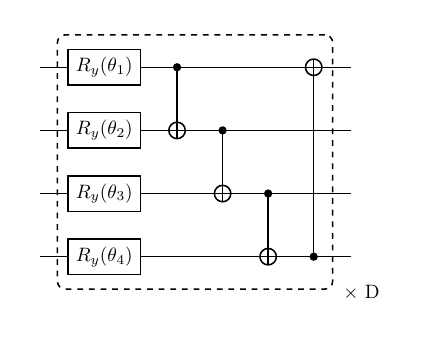
\begin{tikzpicture}
\node[scale=0.7] {
\begin{quantikz}
\qw & \gate{R_y(\theta_1)} \gategroup[4,steps=5,style={dashed,rounded
corners,fill=blue!0, inner
xsep=2pt},background,label style={label
position=below right,anchor=north,xshift=0.7cm,yshift=-0.0cm}]{{$\times$ D}} & \ctrl{1} & \qw & \qw & \targ{} & \qw  \\
\qw & \gate{R_y(\theta_2)} & \targ{} & \ctrl{1} & \qw & \qw & \qw  \\
\qw & \gate{R_y(\theta_3)} & \qw & \targ{} & \ctrl{1} & \qw & \qw  \\
\qw & \gate{R_y(\theta_4)} & \qw & \qw & \targ{} & \ctrl{-3} & \qw
\end{quantikz}
};
\end{tikzpicture}

\end{document}